% !TEX root = ../../thesis.tex

% \cleardoublepage
% \newpage
% \thispagestyle{plain}
% \mbox{}
% \includepdf{/Users/matthieulapeyre/Documents/phd_thesis/media/thebeast.pdf}
\chapter{Robot morphology: some facinating work} % (fold)

\cleanchapterquote{The cognition needs a body to think}{Rodney Brooks}


\section{The emergence of embodiement} % (fold)

In 1949, the Elmer and Elsie robots, also known as turtle robots (see \figurename~\ref{fig:walter_robot}), created by the cybernetic pionner W. Grey Walter, can be considered as one of the first robot in the modern era of the robotics history (1950-now). At this time, calculus was done with mechanical machine (see the focusbox) and the transistor was just invented (1948) and computer science was at the begining of numerical era. So the turtle robot was enterely anaglogical and was able to demonstrate complex behaviors (see \figurename~\ref{fig:turtle_behavior}). Whitout any "reflexion" or internal representation of itself and the world, this robot, thanks to its conception and the direct analogical interaction between sensors and actuators was able to avoid abstacle and reach its charing station (Guy Walter, 1949). These complex behavior which we can found in nature were in fact whitout any kind of intelligence and were emergent from the actual morphology i.e. where are placed sensors how they are connected with actuators.

\begin{figure}[]
\centering
    \subfloat[][]{\label{fig:walter_robot}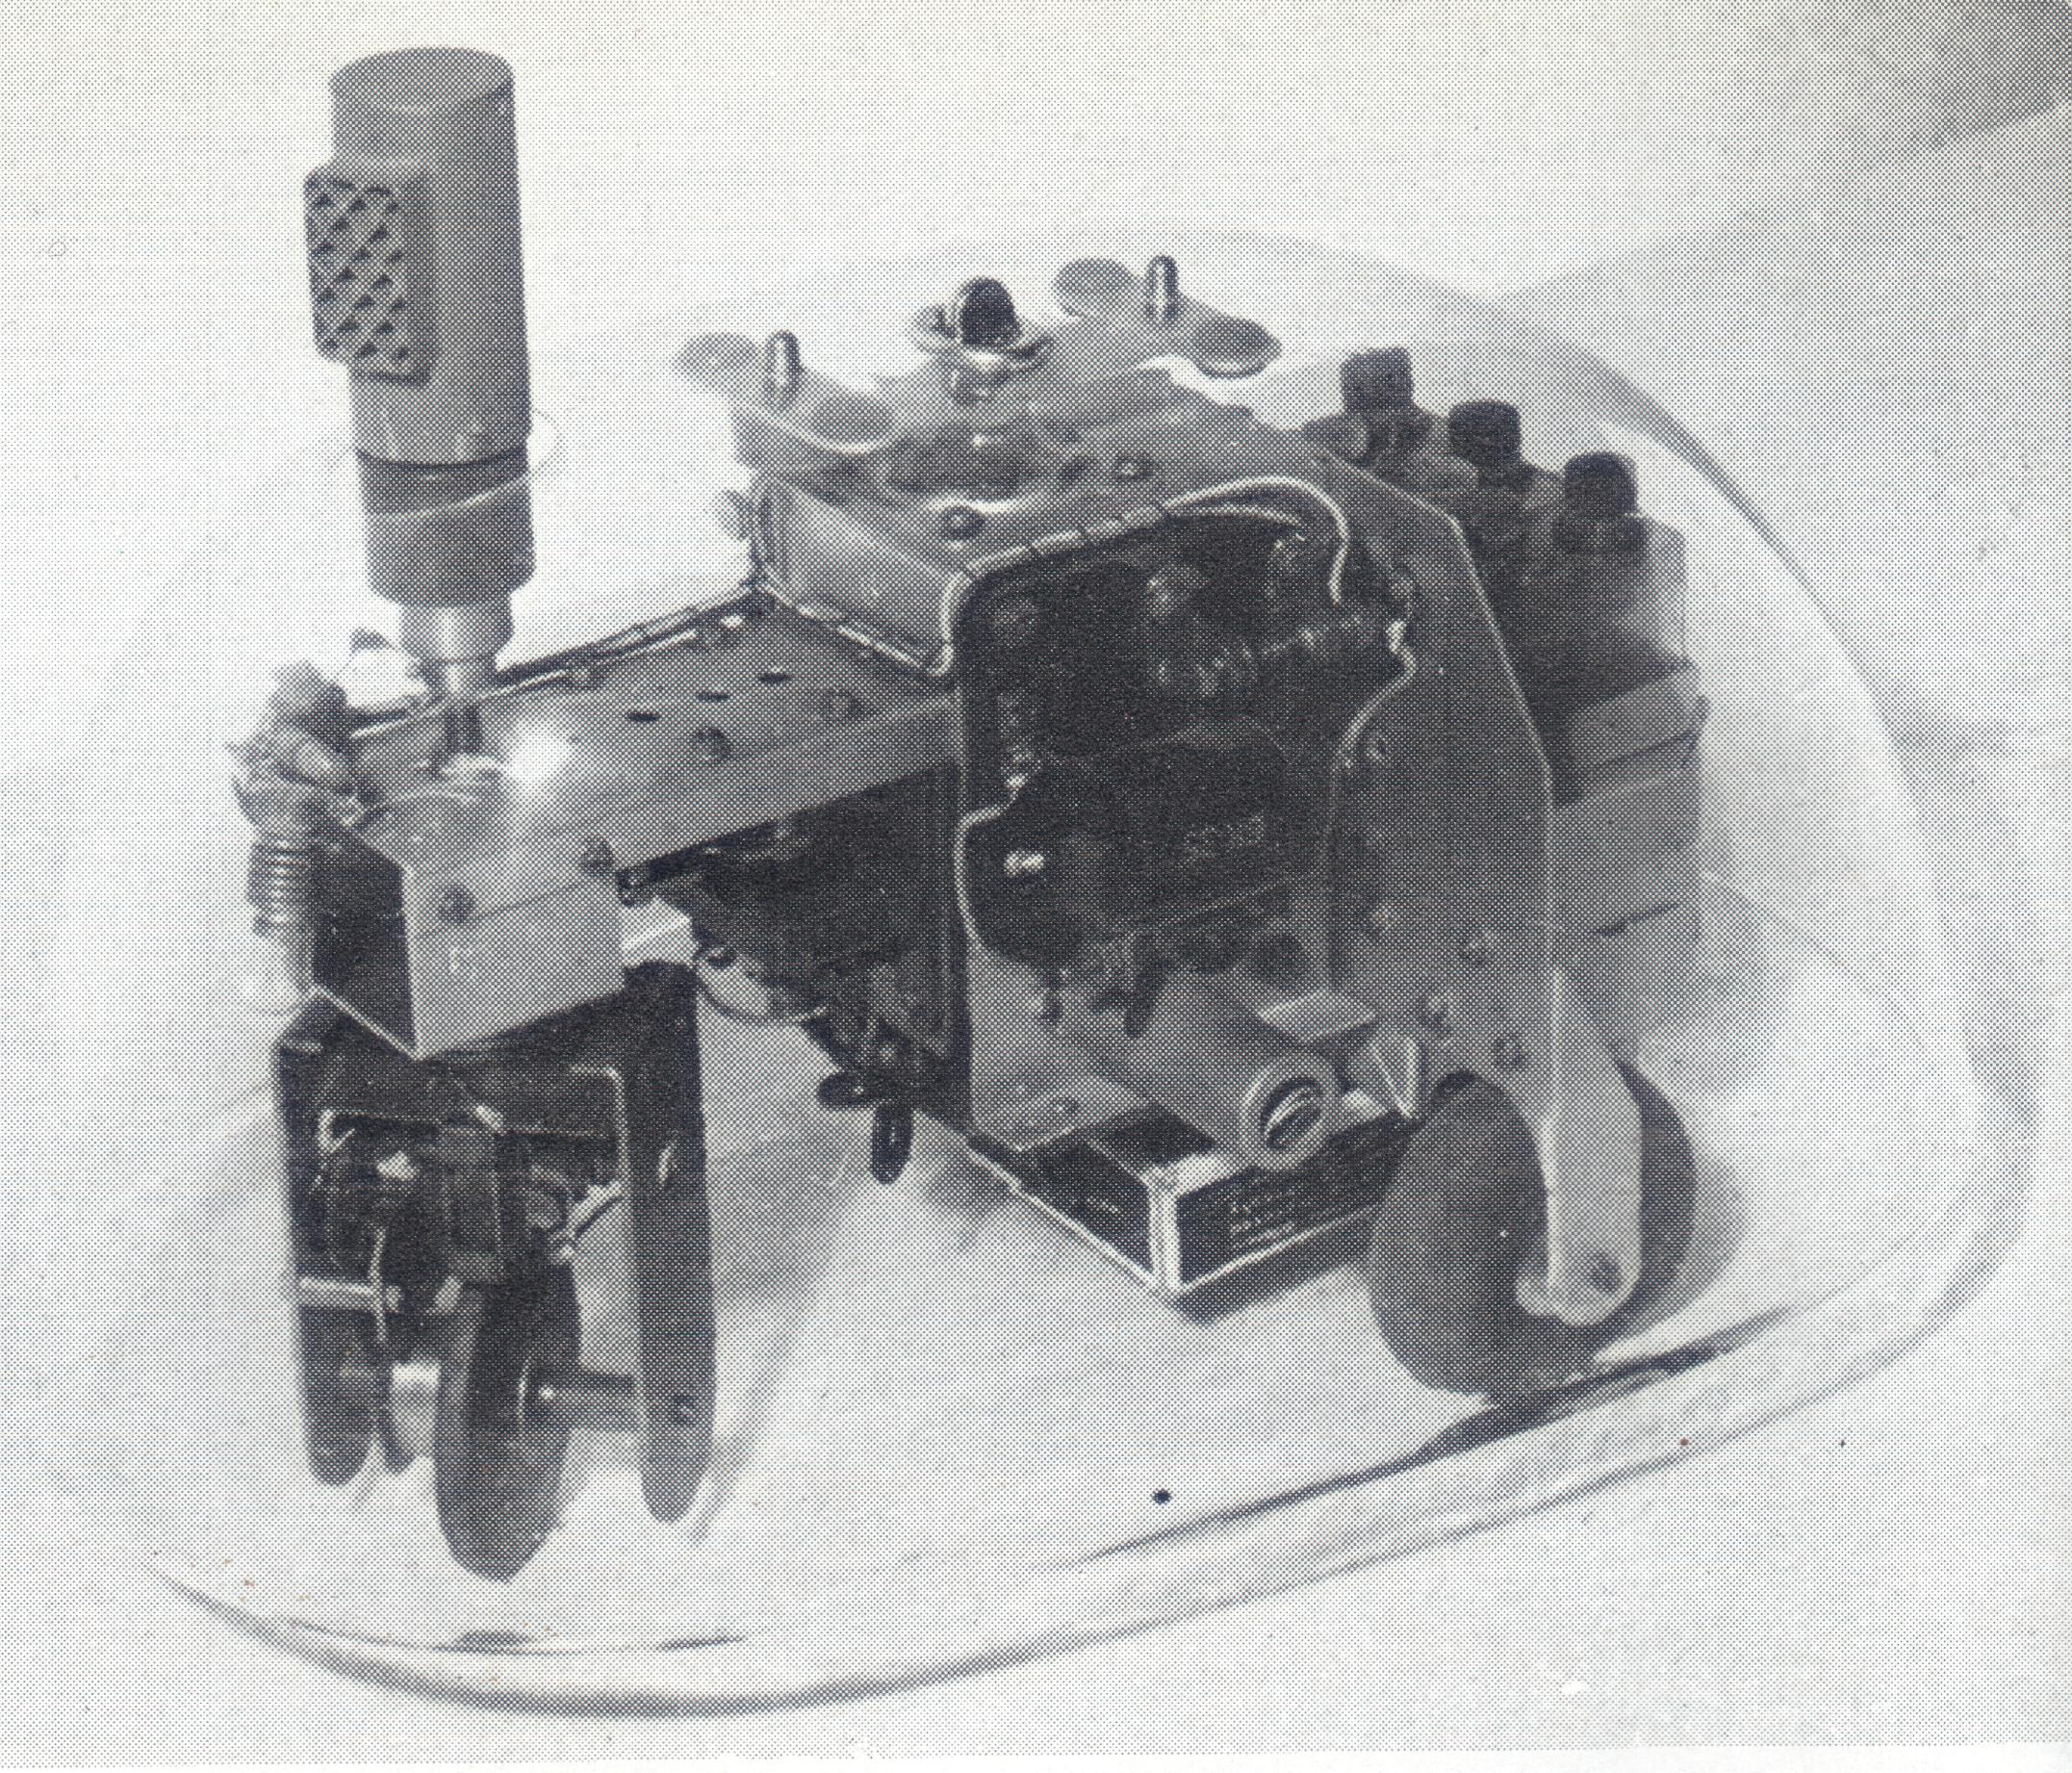
\includegraphics[height=6.5cm]{walter_turtoise_robot.jpg}}
    \hfil
    \subfloat[][]{\label{fig:turtle_behavior}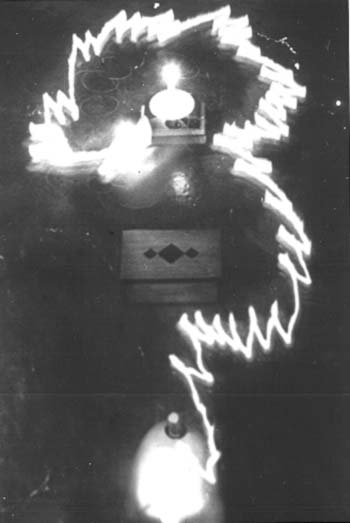
\includegraphics[height=6.5cm]{turtoise_behavior.jpg}}
    \caption{}
    \label{fig:turtle_robot}
\end{figure}

\begin{figure}[]
    \centering
    \begin{boxedminipage}{0.95\textwidth}
        \textbf{Mechanical calculus}\\
        Once upon a time, in a age transistors were not here, complex calculus was done using mechanical properties.
        Using complex mechanisms the very first calculators were fully mechanical machine (see \figurename~\ref{fig:mechanical_computer}).

        The first freely programmable, binary, floating-point, general-purpose mechanical computer in the world was the Z1 constructed by Zuse between 1936 and 1938 (see \figurename~\ref{fig:zuse_z1}).
        This "computer" contained approximately 30,000 components and was incredibly sophisticated, making the Z1 suitable for a wide variety of engineering and scientific applications.
        Introduced by Curt Herzstark in 1948, the Curta (see \figurename~\ref{fig:curta_calculator}) is a small, hand-cranked digital mechanical calculator.
        It can be used to perform addition, subtraction, multiplication, division, and (with more difficulty) square roots and other operations.
        The Curta's design is a descendant of Gottfried Leibniz's Stepped Reckoner and Thomas's Arithmometer, accumulating values on cogs, which are added or complemented by a stepped drum mechanism.
        It has an extremely compact design: a small cylinder that fits in the palm of the hand.

        These two examples show that even pure calculus is acheivable using only morphological properties (here mechanical) and was used during dozens of years for scientific applications.


        Curtas were considered the best portable calculators available until they were displaced by electronic calculators in the 1970s.

        \begin{center}

            \subfloat[][Zuse Z1 (1936)]{\label{fig:zuse_z1}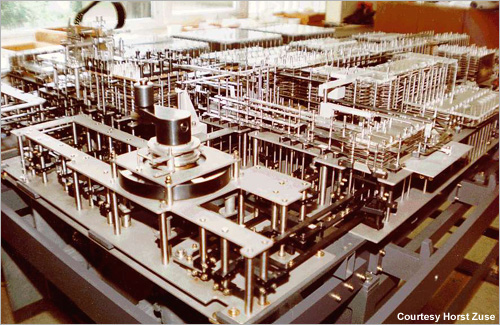
\includegraphics[width=0.42\linewidth]{hist-z1-reconstruct.jpg}}
            \hfil
            \subfloat[][Curta]{\label{fig:curta_calculator}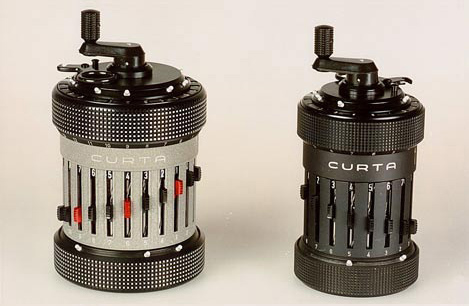
\includegraphics[width=0.42\linewidth]{curta_calculator.jpg}}
            \caption{Mechanical calculus machines}
            \label{fig:mechanical_computer}

        \end{center}

    \end{boxedminipage}
\end{figure}

With the arrival of numeric computer, researchers imagine the opening of a field where it could be possible to replace pre-wired analogic electronical behavior by using computer running program which is therefore more polyvalent because not dependent on the hardware platform. The artificial intelligence term was introduced in a workshop organized in 1956 by a MIT professor John McCarthy. Globally participant were convinced that by using the notion of computation or abstract symbol manipulation it would be possible to reproduce interesting abilities similar to human ones (McCorduck's Machins who think, 1979) (Haugeland, 1985) . The symbol-processing paradigm or cognitivistic paradigm see the cognition as pure computation. In other word, the relevant intelligence process is the abstract algorithm or the program. Eventually, researchers following this paradigm no longer saw the physical incarnation as a relevant component. Cognitive and computationalists hypotheses stating that the thought is reducible to a set of symbolic calculations are being etablished (Fodor, 1987). The body, for its part, is forgotten, irreparably separated the mechanisms of intelligence \cite{kaplan2008corps}. More thant that, the real world body is non perfect, there is noise on sensors acquisition, there is gravity, friction and inertia acting on actuators and the environnemnt is always changing and unpredictable. The robot body became a handicap which often ruins the efficient of algorithm and program created by AI researchers.

To overcome these issues of real world application, the other side of the robotics community, still interested in the hardware challenges work strives to design more reliable and powerfull robot which can react as close as possible as the model used for its control. To do that, it is needed to have way more precise sensors and powerfull enough actuators to counter-act the motion inertia and mechanical friction. Thanks to these research on hardware, industrial robots became more and more fast and precise, enough to outclass any human on specific assembly tasks.

However, even with real efficient robot, artificial intelligence fail to show results comparable with the expectations researcher and society had. Robots are able to solve incredebly complex task such as chess game or able to produce high precision task in manufacture but require perfectly controlled and predictable environment. Going outside this known environment seems impossible to program and none of them is able to act fluently in the real world.

Classical approach known great successes to solve abstract problem such as chess game, search engine, text processing, however it failed in the understanding of natural forms of intelligence which requires a direct interaction with the real world. This is especially the case when we think in the current state of the art for interaction with human (natural langage) or object (grapsing) and the locomotion in an open environment (walk, run, ride a bicycle).

Stucked with these major issues raised by the real world, a kind of crisis of the artificial intelligence happened in the 1980's and the cognitivist paradigm is questionned. While some researchers of the field use new tool such as neuronal networks, another part question the "cognition is computation" approach and the irrelevance of the body. Thanks to researcher such as Rodney Brooks~\cite{brooks1991intelligence}, Rolf Pfeifer~\cite{pfeifer2001understanding} or Luc Steels~\cite{steels1995artificial}, a novel paradigm emerge: the cognition needs a body to think. The embodied artificial intelligence rejects the symbolic approach and postulates that it is not possible to have intelligence without the body and the environment~\cite{pfeifer2001understanding}. Rather than postulating there is a hierarchical structure in which the brain control the body, the new theory focuses on the interaction between the two systems, even for mathematical thinking we could assume is purely abstract (Lakoff and Nunez).

Following this paradigm, researchers try to tackles challenges in which the classical cognitivist approach failed i.e. the understanding of natural forms of intelligence which requires a direct interaction with the real world. The locomotion is a great example of task where the classical robotic approaches globally failed. Animals are incredibly skilled, even if we take insect with a brain thousand of times smaller than the human one, their abilities to move in an open world is just incomparable with the most advanced current robot. One important reasons for this is that in the classical view, the ability to figure out where you are is based in detailed inner models or representaiotns either have to be programmed into the robots or learn by interacting with the environnement and continously updated. The more complex these models are, the more effort is needed to accquire the relevant data to maintain them leading to major problem when learning task in a high dimensionnal space (plein de ref). rooks argued in (1991a) that intelligence always requires a body and that we should forget about complex internal representaitons and models of hte outside world; that we should not focus on sophisticated reasoning processes but rather capitalizer on the system-environment interation. Then he started to work on the insect locomotion () because if we understand the insect-level-intelligenec it will be much easier and faster to understand and build human-level intelligence.

\textbf{TODO: petite review du boulot de brooks avec les insects}

Exploring the role of the morphology and it shape the ways we think appears as a fascinating open field. Exploring the interaction between body properties and cognition could lead to both a better understanding of animals’ behaviour (human being in particular) and to build robot more adapted and robust to an open environment with unpredictable interaction.

Thus an interesting evolution of the last decades is the demonstration of the importance of the morphology for sensorimotor control, cognition and development. The researches community exploring the emboiement paradigm has grown but surprisingly not as muche we could imagine with classical paradigm fails. However, new work arised introducing new principles, we will describe in this chapter, such as morphological computation, compliance or ecological balance, emergence.

In the context of this thesis we will talk about intelligence with the meaning, ability to move in a natural environnment and interact with people and objects.

\section{Morphological computation} % (fold)

As we saw in the introduction, with the arrival of numeric computing, the interest for the robot body seemed less and less revelevant for artificial intelligence reserachers. For them, the "think is calculate", this leads to the cognitivist approach which globally failed in the understanding of natural forms of intelligence which requires a direct interaction with the real world.
However, while we can think there are indeed calculus necessary to achieve complex task, there is no reason it should explicited with a precise internal model or representation of the physical world. It could directly be done by the body properties. The principle is called morphological computation, meaning computation obtained through the interactions of physical form with the ecological niche environnement.

Following the definition of the robotic morphology given by C.Paul:
\begin{quotation}
The morphology of a robot thus refers to the physical structure and form of a robot. Specifically, the focus is on characteristics such as link sizes, number of links, joint characteristics, mass distribution, actuator characteristics, material properties, sensor characteristics and sensor placements. In short, any characteristic which defines the physical structure of the robot is included in the term morphology.
\signed{Chandana Paul~\cite{paul2006morphological}}
\end{quotation}

We are particulary interested in this thesis in the role of morphology for the locomotion and interaction in the human ecological niche.

For decades and it is still mostly the case, the challenge of locomotion for robotic agent was only tackles through symbolic abstract and complex computation of internal model and representation of the world. However, regarding the nature, it appears obvious that an animal morphology deeply change the way it can act in its ecological system and so it has evolved trying to optimize its body properties. For example, it seems evident that the duck has palm feet to improve is swimming ability while primate have hands which allow agile locomotion through the trees.

For some reasons, in the robotics and artificial intelligence field the link between the body properties and the ability for a robot to move in an ecological environnement does not seems as obvious. The fact that the ability to do thing is due to the brain computation is so deeply grounded than it affects even the general public.

Since the 80's, the fact that the morphology of a robot affects its control requirements has become increasingly evident in robotics. Not only does the morphology determine the behaviors that can be performed, but also the amount of control required for these behaviors. Particularly in systems where behavior is obtained through purely sensory-motor interactions of the body with the environment, the morphology is of prime importance. Nonetheless, even in other robotic systems, a relationship has been found to exist between morphology and control requirements, in that some morphologies yield themselves to being more easily controlled than others.

This relationship was first observed and characterized by Pfeifer as the morphology and control trade-off ~\cite{pfeifer2001understanding}, but the mechanisms underlying this relationship have been unclear. The fact that simple physical interactions give rise to computation indicates the theoretical possibility for the dynamics of the morphology to play a computational role in the system, and thereby to subsume part of the role of control~\cite{paulinvestigation}

However, beyond the animal kingdom evidence, the human being already understood this principle in other domains. As in this thesis we are more concerned about the locomotion, we can cite all the vehicules allowing human to locomote in various way invented. Most of the vehicule we used today were invented before the apparition of computer science and were totaly functionnal without any kind of explicit computationnal intelligence.

A car, for example, is an autonomous system able to move in wide range of environnement from perfect asphalt circuit to deep jungle mainly thanks to the damper it has. There is no computaiton of the correct wheel position given a model of the external world and a planning path. The position is just due to the interaction of the car damper properties and the ground.

Another great example is the plane. Make a machine fly is one of the great scientific and engeenering example acheived thanks to a deep understanding of the interaction between the environnement and the morphology.

% For decades (and it is still the case) roboticists try to solve the locomotion, in particular the biped one with complex behavior based on high-speed full dynamics calculus of internal model. But if being able to move was only a question of intelligence, flying should note be a problem for us. We are way more intelligent than a fly, we should be able to it easily !

% Anyone saying that will look kind of idiot in front of its audience, no ? However, given the current robotiscist approach, it is somehow logical. If being able to act in the environnement was only a computational problem, then anyone more intelligent, meaning able to perform more calculus, than a flying creature should be able to fly.

% Of course, it does not make any sense and we understand easily why. Even a really intelligent creature needs a body to actually fly. With our currently biased point of view it would be even difficult to imagine a flying creature whitout proper wings.

% More than that, the actual achievement of the fly does not require any computation. Everything needed is described by the nature law expressed by Bernouilli and an adapted morphology. It is pure morphological computation and it allows to achieve a locomotion as complex as the fly !

\subsection{the fly} % (fold)

If we study a complex behavior such as the ability to fly. Using a cognitivist paradigm, the fly would require a large amount of explicit calculus.  With this approach we could think the fly need a large amount of explicit calculus. However the aeronautic people already understand that the plan they are trying to make fly will act in the real world and the real world is the "air". A plane can only fly because of the air and because it is viscous. The air is not a constraints it is the central element for make a plane fly.

Indeed a plane has to deal with its environnement which is the "air".

While ones could see the real air as a constraint because of its viscousness and prefer model it as a perfect fluid in simulation, it would be impossible or at least way more complicated to make a plane fly. Indeed, it is because the air is viscous that the fly is possible.

Actually a plane fly only thanks to the interaction between its specific wing morphology and the environnment fluid which is the "air".

\begin{equation}
    F_{lift} = \frac12 \times \rho \times V^2\times S \times C_z
\end{equation}

To create lift, the only variable are the profil shape which give the $C_z$ parameter and the surface voilure $S$ and the air properties with its volumic mass $\rho$ and the velocity of the flux $V$.

\begin{equation}
    adapted morphology + air = fly
\end{equation}


All the intelliegence is centered around the wing shape.


Another great example of how mechanics properties can produce complex behavior is the airplane.
The lift force generated by wings are the resulting of the interaction between a air flux and the physical profil shape of the wing.
Then the Bernouilli law add the necessary magic around to make plane fly (see \figurename~\ref{fig:magic_plane})

we can change the behavior by hanging the wing shape, some fighter have a voilure variable

To resume, a plane can work thanks to the fact the air is not a perfect fluid and because it has an adapted morphology. Even rocket use aerodynamic to improve the stability otherwise it would be really complex to keep a direction.



The only way to make machine "fly" without these specificities is to create a rocket which need a very high power to oppose the gravity and complex control to

\begin{figure}[tb]
    \begin{center}
        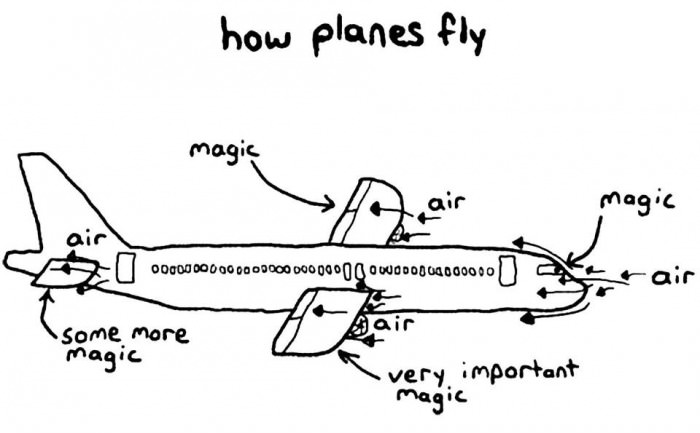
\includegraphics[width=0.8\linewidth]{plane_explanation.jpg}
    \end{center}
    \caption{Caption here}
    \label{fig:magic_plane}
\end{figure}

\begin{figure}[]
\centering
    \subfloat[][]{\label{}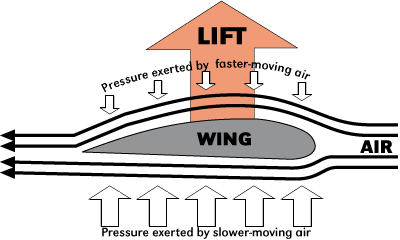
\includegraphics[width=0.56\linewidth]{bernoulli_wing_lift.png}}
    \hfil
    \subfloat[][]{\label{}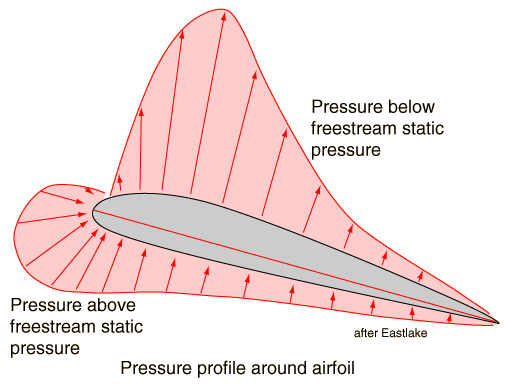
\includegraphics[width=0.42\linewidth]{airfoil_bernouilli.png}}
    \caption{}
    \label{fig:}
\end{figure}

After 60 years of fly history with hundreds of actual plane from planneur to airbus A380, it looks obvious that the shape of the plane is a major, or event the most important part. However, then discussing of legged locomotion, from centipedes to biped ones, the question of the morphology is often left aside in favor to computationnal model. Is there really a fundamental reason the body should be irrelevant for legged locomotion while being essential for flying? There is a lot of legged animals and they are not smater than the flying or swimming ones. Is there a fundamental law comparable to the Bernouilli one ? It can be a biological, a mechanical or even a chimical law, yet it deserves to be explored.

While the velocity of legged locomotion are in most of the case quite low, we could ignore air friction, then a first track could be the interaction between the newton's law and the ground. Using gravity as an advantage instead of a force we have to battle.

\subsection{Passive and Semi-Passive Walkers} % (fold)

This set-up the work of Tad McGeer, comming from the aeronautic field, he was surprised by how the actual legged robot morphology was neglected. A great example is the Tad McGeer's passive walker. Thanks to the understanding of the intrinsic dynamics of its structure, Tad McGeer has managed to create a 2D biped robot capable of producing several steps without any controller or motor showing that such a complex task can be indeed achieved only with adapted morphology\cite{mcgeer1990passive}.

The result is comparable to the sailplane or the paper plane. Using a specific mass repartition and foot shape interecting with gravity and the ground ...

The role of morphology in robot biped locomotion has been particularly explored through the research on passive dynamic walkers~\cite{wisse2007passive}.
The most famous example concerns the Tad MacGeer's work~\cite{mcgeer1990passive}.
Thanks to the understanding of the intrinsic dynamics of its structure, McGeer has managed to create a 2D biped robot capable of producing several steps without any controller or motor.
The only control of this robot is obtained through the interaction between the intrinsic inertia of the structure and gravity.

\begin{figure}[]
\centering
    \subfloat[][Tad McGeer with his prototypes]{\label{fig:tad_mcgeer}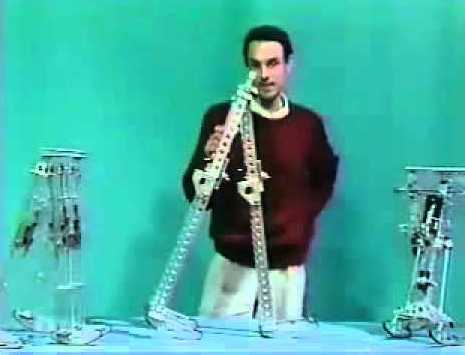
\includegraphics[width=0.49\linewidth]{tad_mcgeer.jpg}}
    \hfil
    \subfloat[][Passive walker robot]{\label{fig:mcgeer_walker}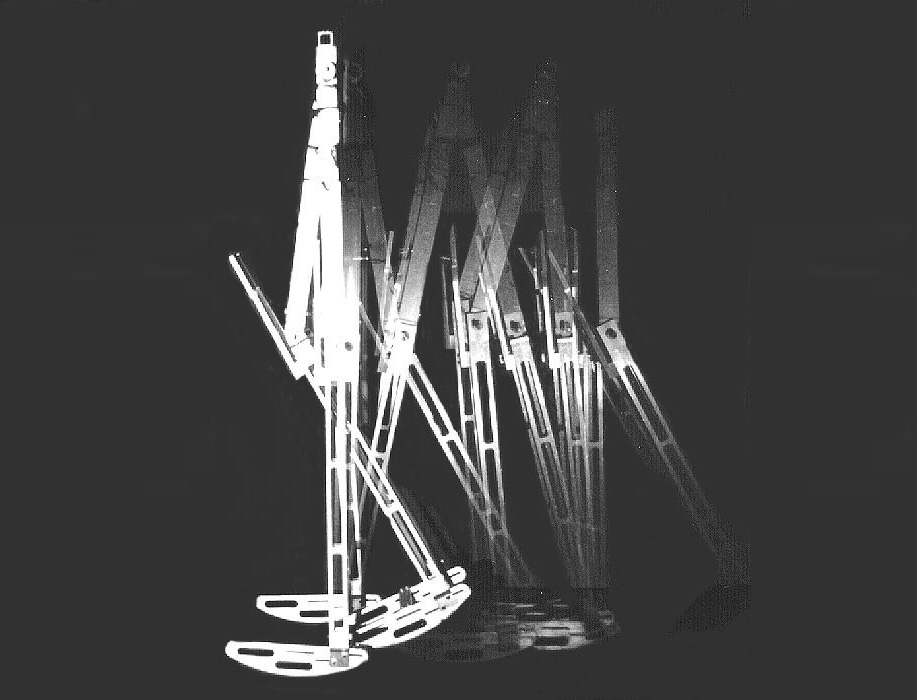
\includegraphics[width=0.49\linewidth]{mcgeer_walker.jpg}}
    \caption{}
    \label{fig:mcgeer_work}
\end{figure}

This work has been pursued with the apparition of semi-passive walker combining both specific passive properties and low power actuation to increase their robustness~\cite{Anderson2005}.
We can note the work of Collins~\cite{collins2005bipedal} which explored the case of semi-passive 3D biped robot.
Its morphology is based on particular mass distribution, knee locking, round feet and springs on the legs to generate an efficient walking gait while keeping its lateral and frontal balance.
The concept of 3D semi-passive robot has been pushed even further with the realization of a complete humanoid robot with trunk, arms and head: the robot Denise~\cite{wisse2005three} and Flame presented in~\cite{Hobbelen2008}.

http://tensegritywiki.blogspot.fr/2010/08/mechanism-as-mind-tensegrity-and.html

we could make a parrallel the energy consumed to th
\begin{figure}[]
    \begin{center}
        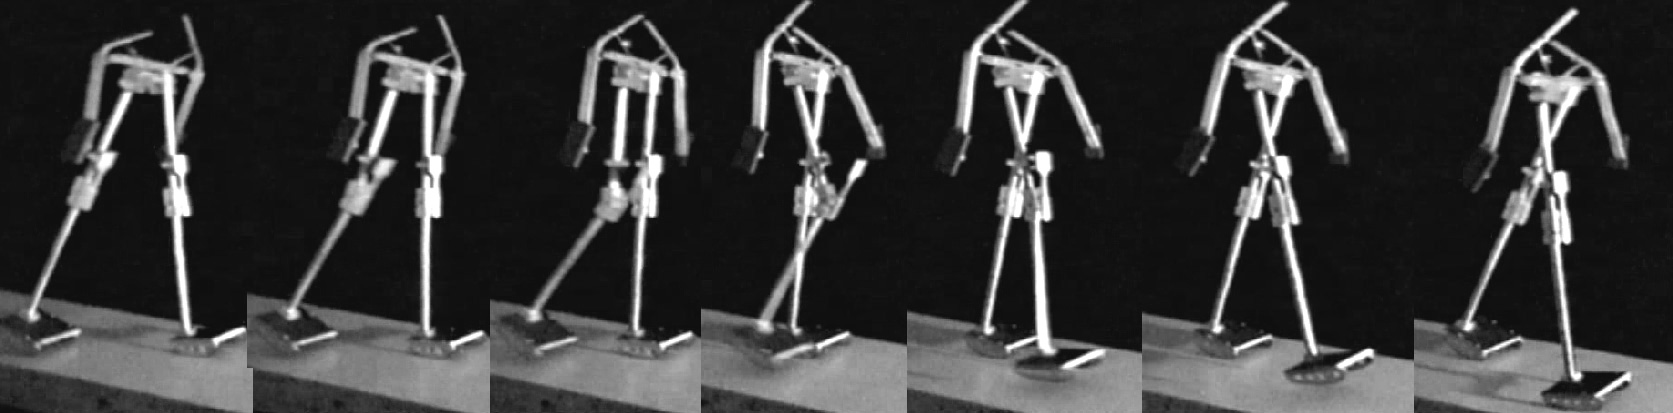
\includegraphics[width=0.99\linewidth]{cornell_biped_series.jpg}
    \end{center}
    \caption{Caption here}
    \label{fig:figure1}
\end{figure}

\begin{figure}[]
    \begin{center}
        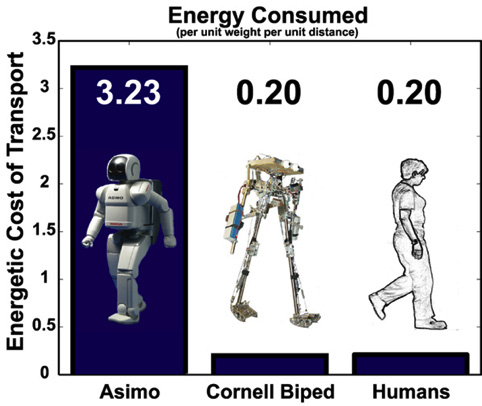
\includegraphics[width=0.6\linewidth]{comparison_cost_transport.jpg}
    \end{center}
    \caption{Caption here}
    \label{fig:figure1}
\end{figure}

\subsection{humans} % (fold)
\label{sub:humans}

% subsection humans (end)
It has also been shown that human morphological properties such as the compliance of the body explains the dynamics of walking and running \cite{Geyer2006} while experiments made by Kojiro Matsushita~\cite{matsushita2005locomoting} show that an adequate morphology is needed if one is interested in natural looking kind of locomotion.


\section{The compliant and soft robotics} % (fold)
It has also been shown that the compliance of the body explains the dynamics of walking and running \cite{Geyer2006} and several biped robots such as Athlete Robot \cite{niiyama2010athlete} or BioBiped1 \cite{radkhah2011concept} were designed using compliant actuator or elastic material.

\section{Ecological balance}

The concept of morphological computation has also been associated to the principle of “ecological balance”, as outlined by Pfeifer et al.\cite{pfeifer2005new}, which states that there is a balance or task distribution between morphology, materials, control, and interaction with the environment.

\section{Emergence of complex behavior} % (fold)

\subsection{Acroban} % (fold)
\label{sub:acroban}
Among all robots designed to explore morphological computation and compliant body only few allow to explore physical interaction such as Kenshiro \cite{Asano2012} or Acroban which the compliant structure of its vertebral column and legs was shown to permit a self-organized physical human-robot interface allowing non-expert users to lead the robot by the hand \cite{Ly2011bio}\cite{Oudeyer2011}.
% subsection acroban (end)

\subsection{Ijspert} % (fold)
\label{sub:ijspert}

% subsection ijspert (end)
PARLER DE LA SALAMANDRE DE IJSPERT
For example, morphological computation has been shown to be necessary in order to achieve human-like biped locomotion \cite{matsushita2005locomoting} and the coupling of adequate morphologies with central-pattern generators has been shown to generate robust locomotor behavior \cite{ijspeert2007swimming}\cite{steingrube2010self}.


\subsection{The sandbeast} % (fold)
\label{sub:the_sandbeast}

% subsection the_sandbeast (end)

Another time, I would like to take a look outside the roboticist community and focus on the work of Theo Jansen.
Theo Jansen is a sculptor in the kinematic art field. Among all his work, he is the creator of the "beast" (see \figurename~\ref{fig:theo_jansen_beast}). These giant structure are moved by a clever mechanism. Composed of eleven small rods, one unique rotation is transformed in walking motion (see \figurename~\ref{fig:beast_mechanism}).

he want to create new form of life which could survive on their own on the beach. The beast get energy from the wind. It can change the direction, it can store energy in limonade bottle and use this energy in case of the wind fade away.

The proportions of the 11 rods is critical to achieve the walking motion

It can "measure" where it is on the beach and avoid going in the sea.

ça peut planter des peieux dans le sable

it can detect obstacle

It walk sideway with the wind in front

He created a brain system with logical door

\url{https://www.youtube.com/watch?v=rWbU3eV4ZpQ}
72 legs moving at the same time using one cranks


\begin{figure}[]
    \begin{center}
        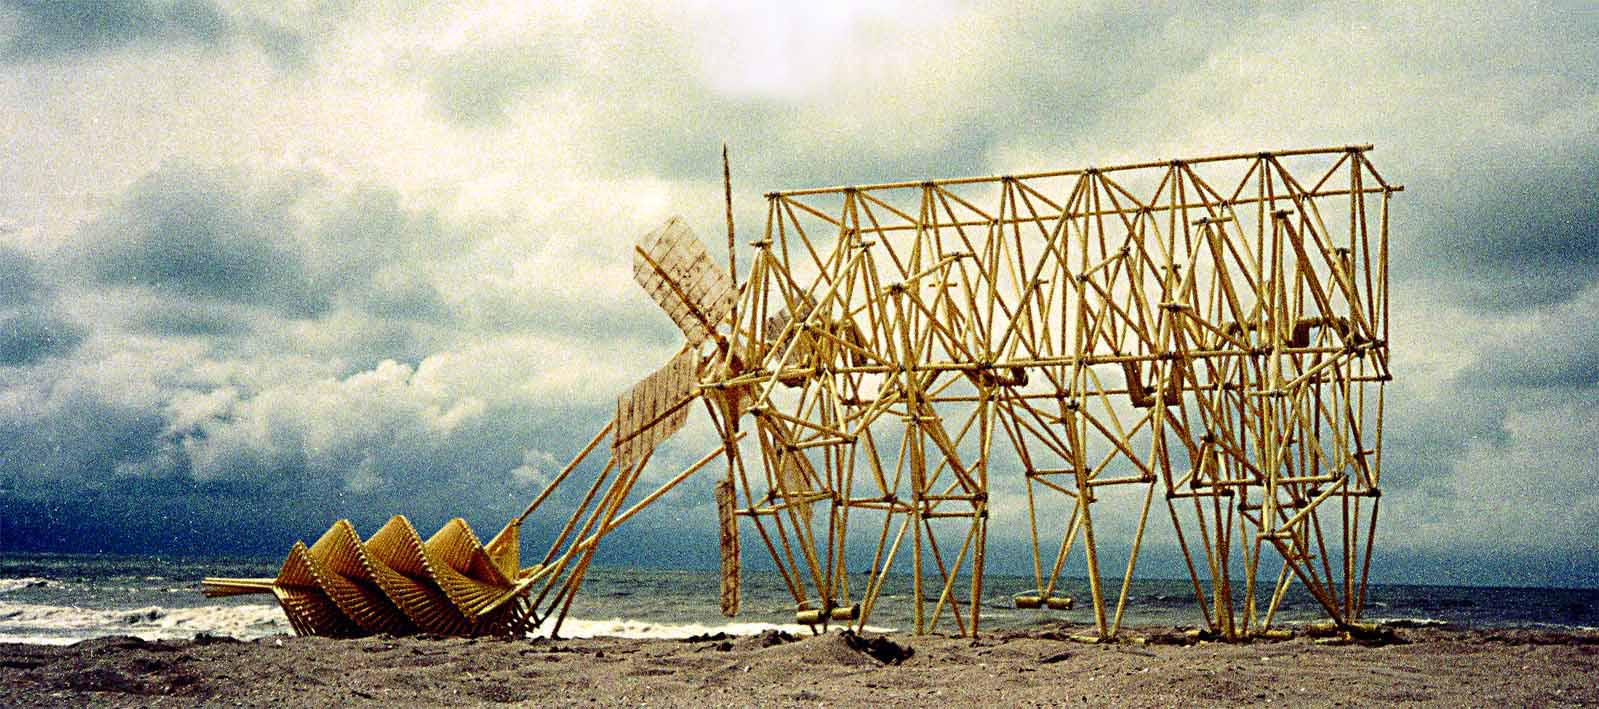
\includegraphics[width=0.99\linewidth]{theo_jansen_beast.jpg}
    \end{center}
    \caption{Caption here}
    \label{fig:theo_jansen_beast}
\end{figure}

\begin{figure}[]
\centering
    \subfloat[][]{\label{}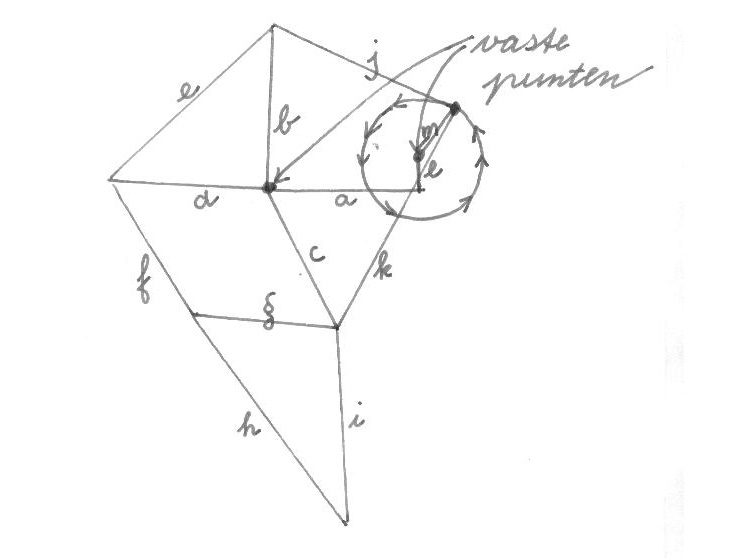
\includegraphics[width=0.32\linewidth]{strandbeest_theory.jpg}}
    \hfil
    \subfloat[][]{\label{}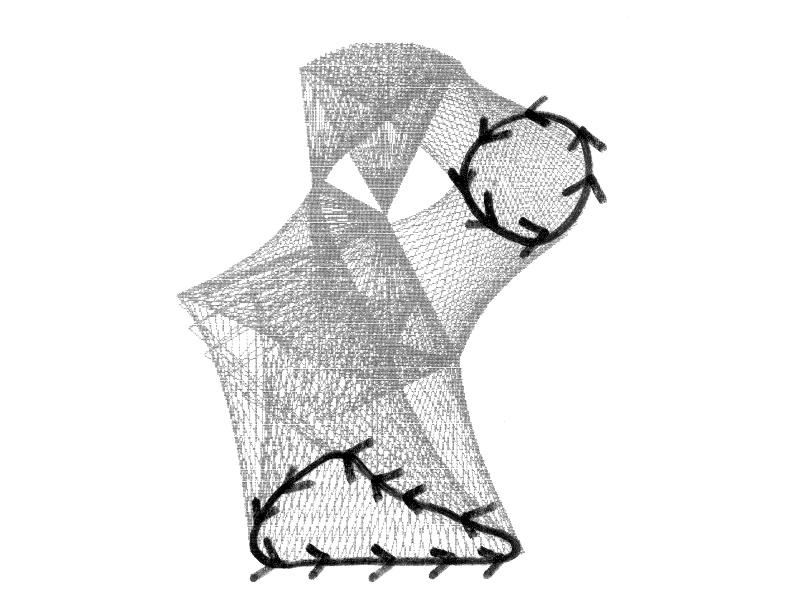
\includegraphics[width=0.32\linewidth]{strandbeest_motion.jpg}}
    \hfil
    \subfloat[][]{\label{}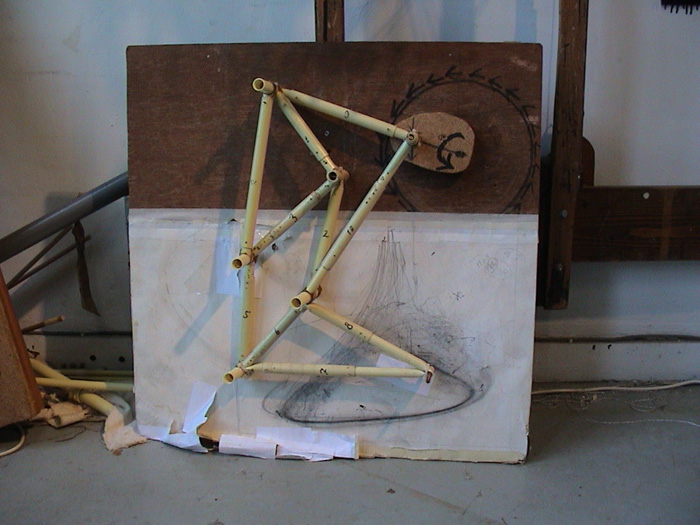
\includegraphics[width=0.32\linewidth]{strandbeest_leg_element.jpg}}
    \caption{}
    \label{fig:beast_mechanism}
\end{figure}


But he is not only interested by the walking, he provides to his beast a morphology allowing them to save energy, avoid stuff, build stuff etc ...

These sculpture are moving on the beach, on the sand,


\section{Exploration de la morphologie dans la robotique} % (fold)




\section{Robotic} % (fold)
For years, artificial intelligence was only considered through complex computation.
An interesting evolution during the last decade was the emergence of work showing the importance of the actual robot morphology in the robot behavior.






These robots showed interesting hopping and running behavior while using less power actuator than common humanoid robot such as Asimo or HRP-2.



The morphological properties of these robotic platforms are especially interesting but unfortunately they are difficult and expensive to reproduce by other research laboratories.
Most of the studies made on the humanoid robot locomotion in the past 30 years~\cite{park1998biped}~\cite{aoi2005locomotion}~\cite{park1998biped} mainly focus on tackling the challenge of biped walking through the active control of the whole robot dynamics using technics such as ZMP control~\cite{vukobratovic2004zero} requiring very precise and high torque actuation~\cite{akachi2005development}.

The properties of the robot morphology have shown interesting results for robust locomotion, for instance the hexapod robot Rhex~\cite{saranli2001rhex}.
Still, it is surprising that only few explored the challenge of biped locomotion through the study of the role of morphology.
One can cite the work of Chandana Paul and Josh C.Bongard~\cite{paul2001road} and Ken Endo~\cite{endo2002co} which have explored evolutionary optimization on robot morphology to achieve stable biped locomotion.
They have showed a strong impact of the morphology on the walking behavior and were able to reduce the complexity of the controller by finding good mechanical properties (limbs length and mass distribution).


\section{Conclusion} % (fold)

Scientific study of the role of morphology in sensorimotor control and cognition: in Robotics (McGeer, Pfeifer and co.), in relation with Cognitive Science (e.g.
http://www.pyoudeyer.com/IEEETAMDOudeyer10.pdf ) and animals (e.g.
work of Robert Full)

EmbedIT – An Open Robotic Kit for Education
\url{http://www.eucognition.org/index.php?page=tutorials}
